\section{Proposed Method}
\label{sec:proposed_method}

% Since the pioneering work of Daugman on iris recognition 
% through texture patterns~\cite{daugman1993high}, different forms of iris texture characterization have been proposed both for iris recognition and for presentation attack detection. 
The task of the PAD algorithm is to capture differences between an actual live iris and either non-iris object, non-conformant use of an actual iris, or a cadaver eye. In the simplest scenario, when only static features of a single iris image are used, the PAD method recognizes anomalies in the presented iris texture. However, given different fabrication processes and the richness of details in an iris, it is likely that any single texture descriptor cannot capture all necessary leads hinting at a possible attack. Therefore fusions of different texture descriptors (\eg LBP, BSIF, Gabor filters) and classifiers (\eg Support Vector Machines, Neural Networks, etc.) have also been explored in prior literature.

Although texture analysis has been a staple in iris research over the years, development of image processing methods that capture such intricate textures has been a challenge. Therefore, more recently some researchers have brought to bear data-driven techniques, especially deep CNNs, to learn directly from training data the 
% appropriate ways how to extract 
iris features useful in PAD. Normally, the input of such networks are the raw pixels themselves. Even though such data-driven methods have led to good results, these models do not work well in the so-called cross-domain setup, \ie when different training/testing conditions are part of the problem. As such, the conditions during training are not enough to allow robust generalization during testing.

This is where our work herein comes into play. In this section, we present a way of accelerating and empowering CNNs to capture texture patterns in such a way that differences among genuine and attack samples can be more easily spotted. Conscious of the representational power of CNNs to properly learn discriminative features, but at the same time of their innate need of large amounts of training data, we facilitate the process of learning by feeding the network with transformed input that highlights texture features important to make a distinction between a live iris and a presentation attack iris. We achieve this by transforming the input image into Binarized Statistical Image Features (BSIFs)~\cite{kannala2012bsif}. Second, 
% allied with our expertise on the problem, 
it is likely that looking at the iris texture patterns from different vantage points, including different scales, might allow us extracting more features capturing differences between authentic iris patterns and artifacts. 

Thus, we consider using multiple BSIF filter sets, characterized by a scale $l$ and a depth $n$ (number of filter kernels in a single set) to create BSIF representations $B_{n\times n \times l}$ for each $(i,j)$ pixel of the original image $I$:

$$
B_{n\times n \times l}(i,j) = \sum_{k=0}^{n-1}b_k(i,j)2^k
$$

where

$$
b_k(i,j) =  
\begin{cases}
    1 & \text{if } s_k(i,j) \geq 0\\
    0 & \text{otherwise}
  \end{cases},
$$

$$
s_k(i,j) = \sum_{u=0}^{l-1}\sum_{v=0}^{l-1} w_{k;n,l}(u,v) I(i+u,j+v),
$$

\noindent
and $w_{k;n,l}$ is the $k$-th filter kernel in the set of filters derived for a given $n$ and $l$. Using original sets of BSIF filters, as proposed by Kannala and Rahtu~\cite{kannala2012bsif}, allows calculating 60 different BSIF representations of a single image. Each of these 60 image transformations is then used by one CNN to learn higher-level features for discriminating authentic and presentation attack irises. Finally, with different learned features at hand, a natural question is how to effectively select the best ones for PAD detection while eliminating the non-representative ones. For this we exploit two different fusion schemes: one based on random-forest feature weighting and meta-learning strategies, and the second relying upon inter-rater agreement measures.

% We bring to bear some important concepts not yet fully explored in prior art.
% In this case, it is likely that the training samples are not sufficient to realize the (in theory) claim of a universal approximator of a neural network.

BSIF kernels included into each of 60 sets were calculated from natural images in a way that maximizes statistical independence of filter responses, and the Independent Component Analysis was used for this purpose \cite{kannala2012bsif}. Assuming that patterns observed in artifacts are statistically independent of textures observed in authentic irises, such decomposition of images, and then building BSIF representations of image based on binarized filter responses, may facilitate calculating PAD-related features from BSIF representations instead of raw images.

While it is theoretically possible to train a CNN to obtain the same filters as BSIF in its first convolutional layer, the cost function and the training process would be significantly different from our goals and would likely require more training data than one normally has for solving a PAD problem. To reduce the amount of training data, we thus transform the images to a new space represented through BSIF operations and this new input serves as an additional transformation layer for the CNNs. As we go toward the output layers in the CNN, such features are further specialized to higher-level representations. The idea is that feeding the network with a transformed input would allow it to more quickly achieve such deeper representations without extensive training. However, some useful features may still not be learned from this transformed space. Therefore, drawing on good results from previous studies in the PAD literature~\cite{Menotti:TIFS:2015, livdet2017}, in addition to learning features from these transformed spaces, we also consider learning features directly from raw image inputs. At the end, with fusion strategies, we can show how such different treatments are complementary and how some of them do not contribute to separate authentic samples from artifacts. The key aspect of our methodology is that different filters learned from transformed spaces capture richer details than just a single representation and translate to better results in the difficult cross-dataset setup, the one in which training and testing conditions are different. 

Finally, we end up with 61 CNN-based predictors: 60 fed by BSIF representations and 1 fed by the raw image. We refer to such complementary CNNs learned with different input representations as multi-view-CNN predictors. Finding the optimal decomposition of the numerous possible configurations of the BSIF filter sets is not straightforward. That is exactly why the combination of CNNs is powerful. 

Since one of the CNN-based predictor operates on a raw image, it is interesting to compare its first-layer filters with those used in BSIF transformation. Visual comparison of these filters reveals some similarities: at a small scale ($3 \times 3$), most of them resemble edge, corner or dot detectors, similarly to what we would expect in the V1/V2 regions of the brain specialized in roughly describing visual inputs through edges and corners. However, BSIF $3 \times 3$ filters and CNN $3 \times 3$ filters are different. This means that the CNN operating on raw images developed its own way to preprocess the images in the first layer when compared to BSIF-based transformation, which may suggest that this predictor is complementary to the remaining 60 predictors, and it is worth using in the fusion.

Fig.~\ref{fig:method_overview} illustrates the main steps in our approach, which are explained in details in the following sections.

\subsection{Feature Extraction}

% In furtherance of obtaining multiple views from a single input, 
We compute BSIF representations by exploiting filter width size ranges from $3\times3$ to $17\times17$, and depth (\ie number of filters in a set) ranges from $5$ to $12$. Fig.~\ref{fig:bsif_examples} shows some examples of BSIF views of the same image presenting an iris with a textured contact lens. Note how different BSIF representations highlight the pattern of a contact-lens.

We use OSIRIS~\cite{othman2016osiris} (version 4.1)~\footnote{Source code is available in \url{http://svnext.it-sudparis.eu/svnview2-eph/ref_syst/Iris_Osiris_v4.1/}} to find the center of the iris in the original (not BSIF-transformed) image. Next, we crop a $260 \times 260$ region around the iris in both the BSIF-transformed images and the original image. These cropped samples are input to the CNNs in the next step. This $260 \times 260$ size is based on the size of iris images in commercial sensors ($640 \times 480$) and the ISO/IEC 19794-6 recommendation for a minimum 120 pixels across the iris diameter.

% \begin{figure}[!htb]
%     \centering
%     \mybox{blue}{
%     \includegraphics[width=0.7\linewidth,
%                      trim=0.6cm 0.5cm 0.5cm 0.4cm]{version_1/graphics/bsif_vs_raw.pdf}
%     }
%     \caption{\newtext{Distribution accuracy distributions of a Linear SVM with different descriptors computed over the \emph{test unknown} partition of each dataset.}}
%     \label{fig:bsif_vs_raw}
% \end{figure}

%
\begin{figure*}[!htb]
    \centering
    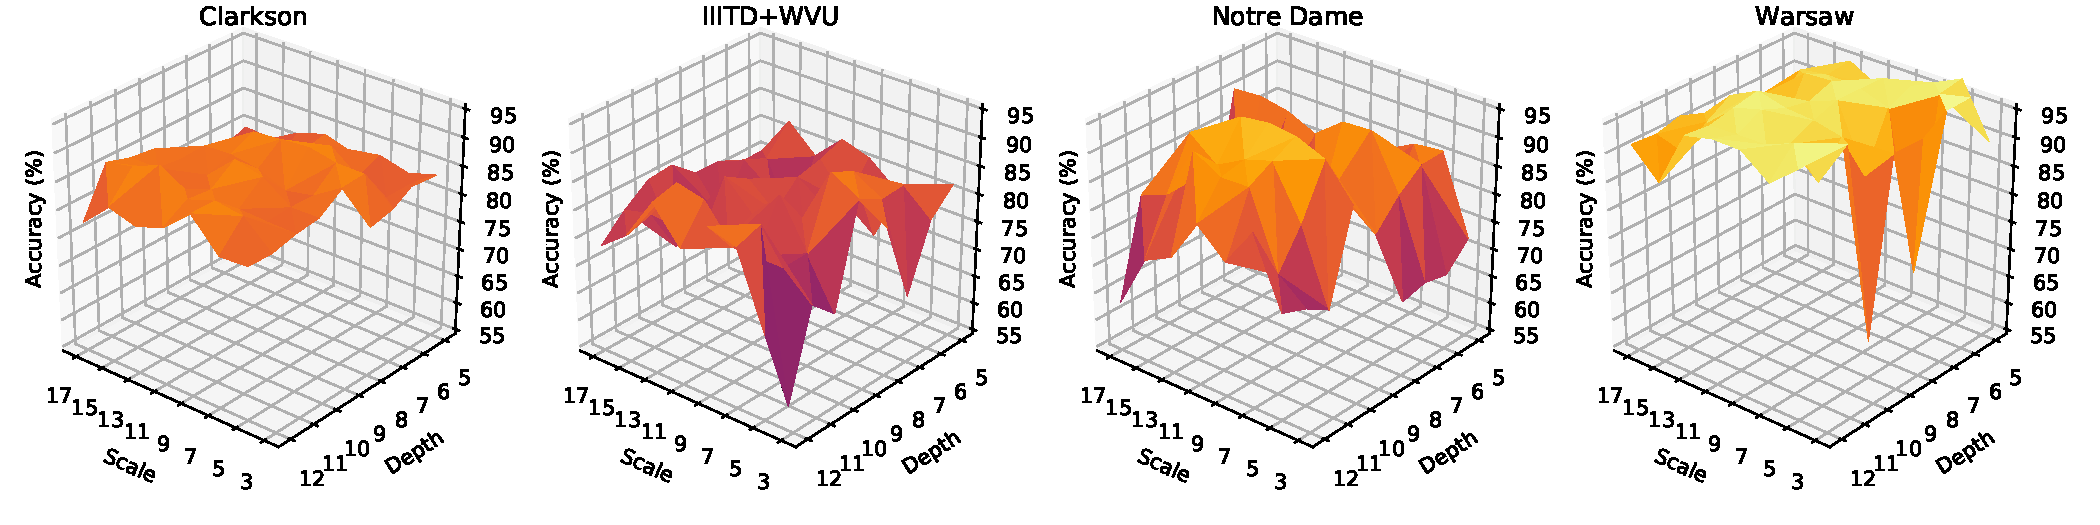
\includegraphics[width=\linewidth,
                     trim=0.5cm 0.5cm 0.6cm 0cm]{bsif_analysis.pdf}
    \caption{Performance comparison of the proposed CNN operating on BSIF inputs of varying scale and depth. Accuracies are estimated over the \emph{test unknown} partition of each dataset.}
    \label{fig:bsif_analysis}
\end{figure*}

To substantiate the descriptive advantage offered by BSIF filtering over the raw image input, we performed a baseline classification using a linear SVM to compare classification accuracies. 
% The distribution of accuracies is shown on Figure \ref{fig:bsif_vs_raw}. 
While the best accuracy obtained with raw images was below 80\%, some of the BSIF filters achieved performance superior to 95\%. 
Besides, the mean accuracy of BSIF images was higher, confirming the potential benefit of  some of the filters.

With the intention of better understanding the results of BSIF images as input features, we performed an ablation analysis on the effect of scale and depth of the BSIF filters on the final classification. A CNN classifier (described in Section \ref{sec:our_cnn}) was trained on different input images, generated by BSIF filtering, first varying filter sizes, and then their depths. Results of this analysis are shown in Figure~\ref{fig:bsif_analysis}. It is possible to observe that some particular scales or depths have some (positive or negative) impact on the classification accuracy, but it is not possible to infer a generalizable trend.

In the same vein, we also tried to vary the size of the filter in the first convolutional layer of the CNN, while training it to perform classification on original images, and compared these results with BSIF (Fig. \ref{fig:cnn_analysis}). In this case, the BSIF classification accuracy was consistently higher, presenting also a smaller variability in the results than the Raw input image. These results suggest a better capability of BSIF filters to capture discriminating features of attack images. Along with the BSIF scale/depth analysis, results  indicate there is a potential gain when using some BSIF filters, and this  encouraged us to develop our fusion strategy explained ahead.

%
\begin{figure}[!htb]
    \centering
    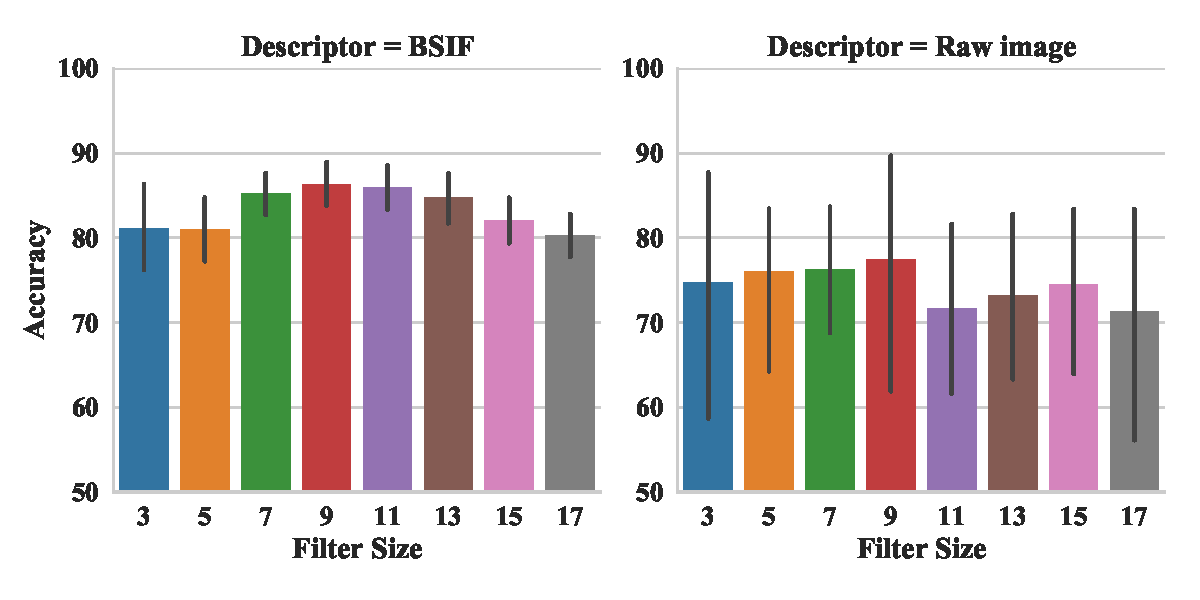
\includegraphics[width=0.98\linewidth,
                     trim=0.6cm 0.5cm 0.5cm 0.4cm]{cnn_filter_analysis.pdf}
    \caption{Performance comparison between BSIF and raw image as the input to the CNN. Accuracies are estimated over the \emph{test unknown} partition of each dataset. The length of the whiskers equals to one standard deviation of the obtained results.}
    \label{fig:cnn_analysis}
\end{figure}



\subsection{Classification using lightweight CNNs}
\label{sec:our_cnn}

%
\begin{figure*}[!htb]
    \centering
    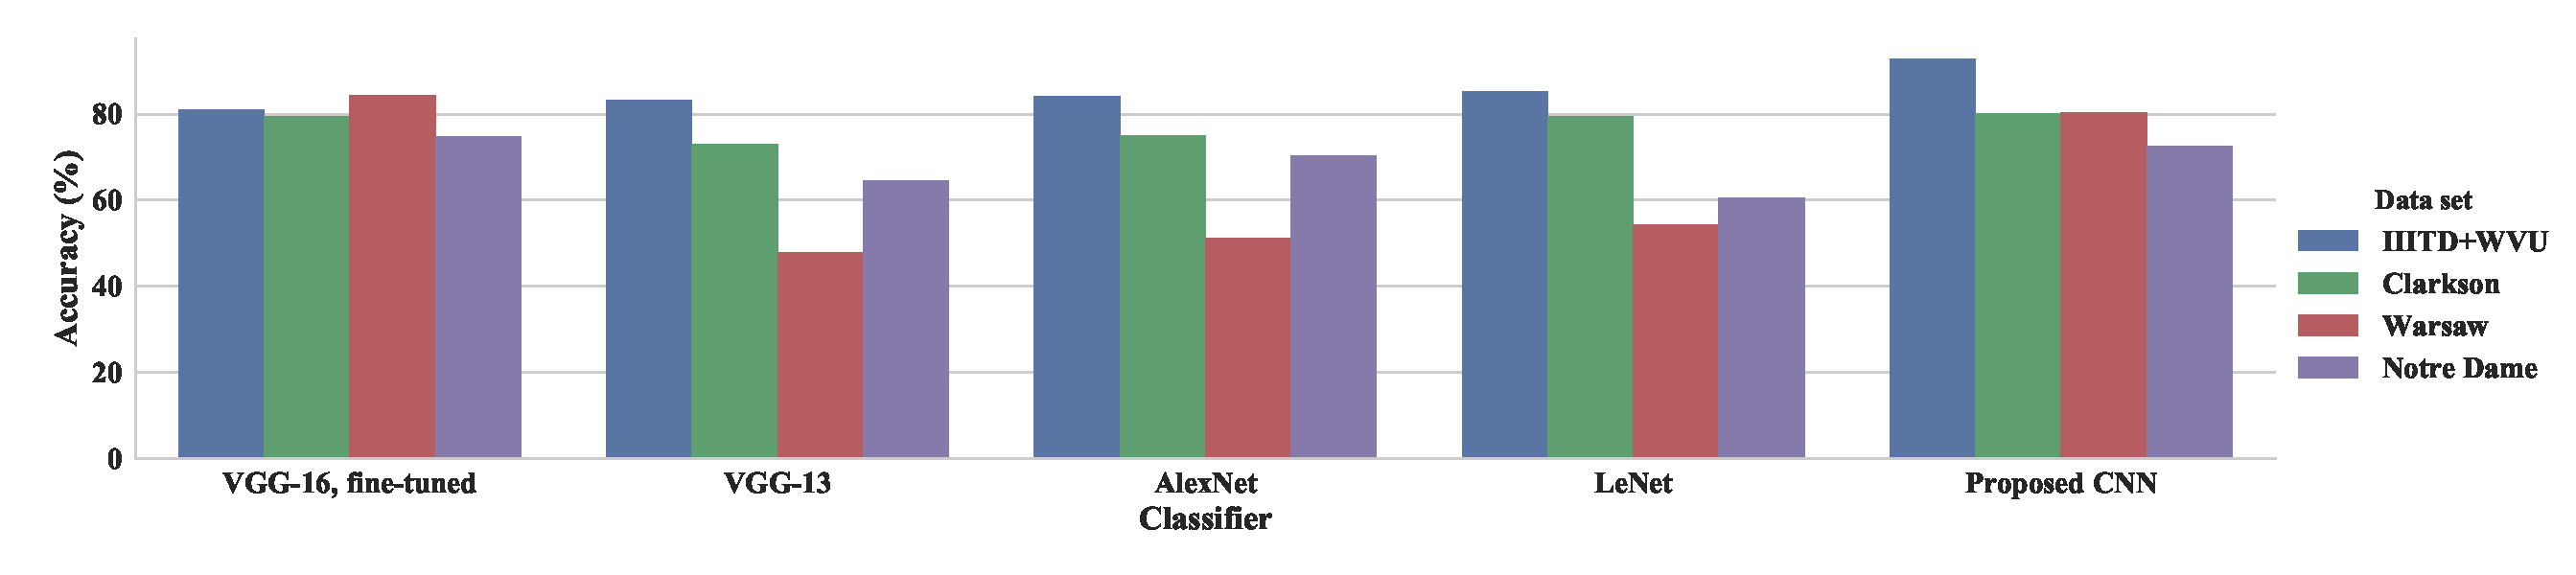
\includegraphics[width=\linewidth,
                     trim=0.9cm 0.7cm 0.5cm 0.5cm,clip]{vgg_analysis.pdf}
    \caption{Performance of CNN architectures on the \emph{test unknown} partition, fine-tuned or trained from scratch in the \emph{train} partition of each dataset. Our proposed architecture has fewer layers, takes less time to train, and results in similar or superior accuracy to other known CNN architectures.}
    \label{fig:other_cnns}
\end{figure*}

As already mentioned, we train a CNN model for each of 60 BSIF transformations of the original image and a CNN for the original image, for a total of 61 CNNs.
As we will show in our experiments, the ensemble of the most complementary CNN models allows us to exploit different aspects of the iris image texture, which is important to achieve high detection rates, especially in challenging scenarios, such as cross-sensor and cross-dataset evaluation protocols.

%A CNN model is trained for each of the 60 different BSIF views of the iris image.
%The BSIF filter width size ranges from 3x3 to 17x17, and the depth size ranges from 5 to 12.
% In order to extract potentially complementary information from different BSIF representations, we trained several CNN models, each one considering a specific BSIF filter size. 
%We believe that this ensemble of CNN models allows us to exploit different aspects of iris image texture. 
%In addition to the 60 CNN models trained on BSIF views, we trained one CNN on the raw iris image.

Given that we do not have large training datasets, and also to avoid possible overfitting to specific datasets through the use of millions of parameters, we opt to use a not-too-deep network architecture. Experiments with deeper configurations did not translate into improved results in our case (Fig. \ref{fig:other_cnns}). Inspired by Menotti~\etal~\cite{Menotti:TIFS:2015}, our CNN architecture comprises two convolutional layers, and two fully-connected layers. Batch normalization~\cite{ioffe2015batch} is applied after each convolutional layer, to optimize the training procedure. The input of the network is an image of configurable size. The first convolutional layer consists of 16 filters of size $3 \times 3$ and Rectified Linear Unit (\emph{ReLU}) activation. Next, MaxPooling on a $9 \times 9$ pixel window and stride 2 is applied, just before the first batch normalization. The second convolutional layer comprises 32 filters of size $3 \times 3$ and \emph{ReLU} activation. 
MaxPooling on a $9 \times 9$ area with stride 8 and batch normalization follow this layer. The output of convolutional layers is fed into a fully-connected layer composed of 1,024 \emph{ReLU} activated neurons. Finally, the output layer is formed by two units, corresponding to two classes we want to recognize (authentic iris vs. presentation attack iris) following the SoftMax transformation. 

\subsection{Ensemble Fusion of Multiple Views}

In this section, we present the proposed approaches for fusing the result of the ensemble of CNNs.
% modeling of the different multi-view-CNN predictors.

\subsubsection{Random Forest Fusion}

Random Forests is a well-known ensemble method that has been used for classifier fusion~\cite{kuncheva2014} as well as for variable importance ranking~\cite{breiman2001random, genuer2010variable}. 
It is composed of multiple decision trees built on different random subsets of the training data.
Some of these decision trees tend to grow deep, sometimes leading to overfitting. This effect can be reduced by balancing the output of the decision trees and through tree pruning. By using a random forest classifier on top of the results of the different multi-view-CNN predictors, we can consolidate their outputs into a single prediction measure. As byproduct of this fusion, the random forest is also able to provide a ranking of predictor's importance, which can help us to select the most relevant predictors for our task.

Random Forests can estimate the test error (generalization error) of the ensemble, without needing to keep a separate test data partition. This is called out-of-bag (OOB) error estimation: the prediction error is calculated on all the samples that are left out of the bootstrap for each of the decision trees. 
During the process of training a Random Forest, after each tree is constructed, OOB error rate (of all variables) is compared to the classification error of the permutation of out-of-bag examples for each of the variables. As a result, we get an estimate of how much the misclassification error increases if each of the variables is disturbed. This measure is called variable importance.


\subsubsection{Voting Fusion}

Another strategy we exploit for decision-making is fusion through voting. We considered \emph{majority} and \emph{weighted voting}. 
% In the majority voting, the number of classifiers predicting each class is counted, and the class with the highest number of votes is selected~\cite{kuncheva2014, kittler1998combining}. 
In its simplest form, 
majority voting~\cite{kuncheva2014, kittler1998combining} considers all 61 CNNs as inputs to decide whether or not a given sample should be considered as an authentic or an attack. The Condorcet Jury Theorem states that if all classifiers produce independent predictions, and if each has a probability of correct prediction that is greater than 0.5, the addition of more voters will increase the probability that the consensus will make the correct decision \cite{kuncheva2014}. Veering away from simple majority voting, in some cases it is desirable to give greater weights to classifiers that are more likely to yield the right decision. With this in mind, we also use a strategy called~\emph{Best-Worst Weighted Vote} (\textit{BWWV})~\cite{Moreno-Seco2006}. The best and the worst ranking predictors are identified and receive maximum and minimum weight (1 and 0, respectively). All remaining predictor weights are linearly cast between these extremes.
%In order not to eliminate the worst predictor from the vote, we attribute a minimum weight to it.

We consider two ways to attribute weights to CNN predictors: classification accuracy and rank importance. For the former, predictors are sorted by decreasing accuracy for the weight assignment. For the latter, predictors are sorted by their rank importance calculated through the Random Forest classifier. We refer to these techniques as \texttt{BWWVA} and \texttt{BWWVI}, respectively.

\subsubsection{Classifier selection and Meta-fusion}
\label{subsec:meta_fusion_algorithm}

One would naturally expect that some predictors provide complementary views on the problem while other predictors are highly correlated.
% , thus just representing noise. 
In this section, we present our proposed algorithm for selecting the most relevant subset of predictors to use as the final ensemble for the PAD. We take advantage of {Gini} importance~\cite{Breiman:1984}, measured with tree-based models, and inter-rater agreement, measured using Cohen's kappa statistic~\cite{Fleiss:EPM:1973}.

Gini importance should give us the most promising predictors in terms of classification accuracy, while the inter-rater agreement measure should give us the most complementary predictors. Fig.~\ref{fig:proposed_method_selection} illustrates the proposed approach.
%
\begin{figure}[t]
\centering
    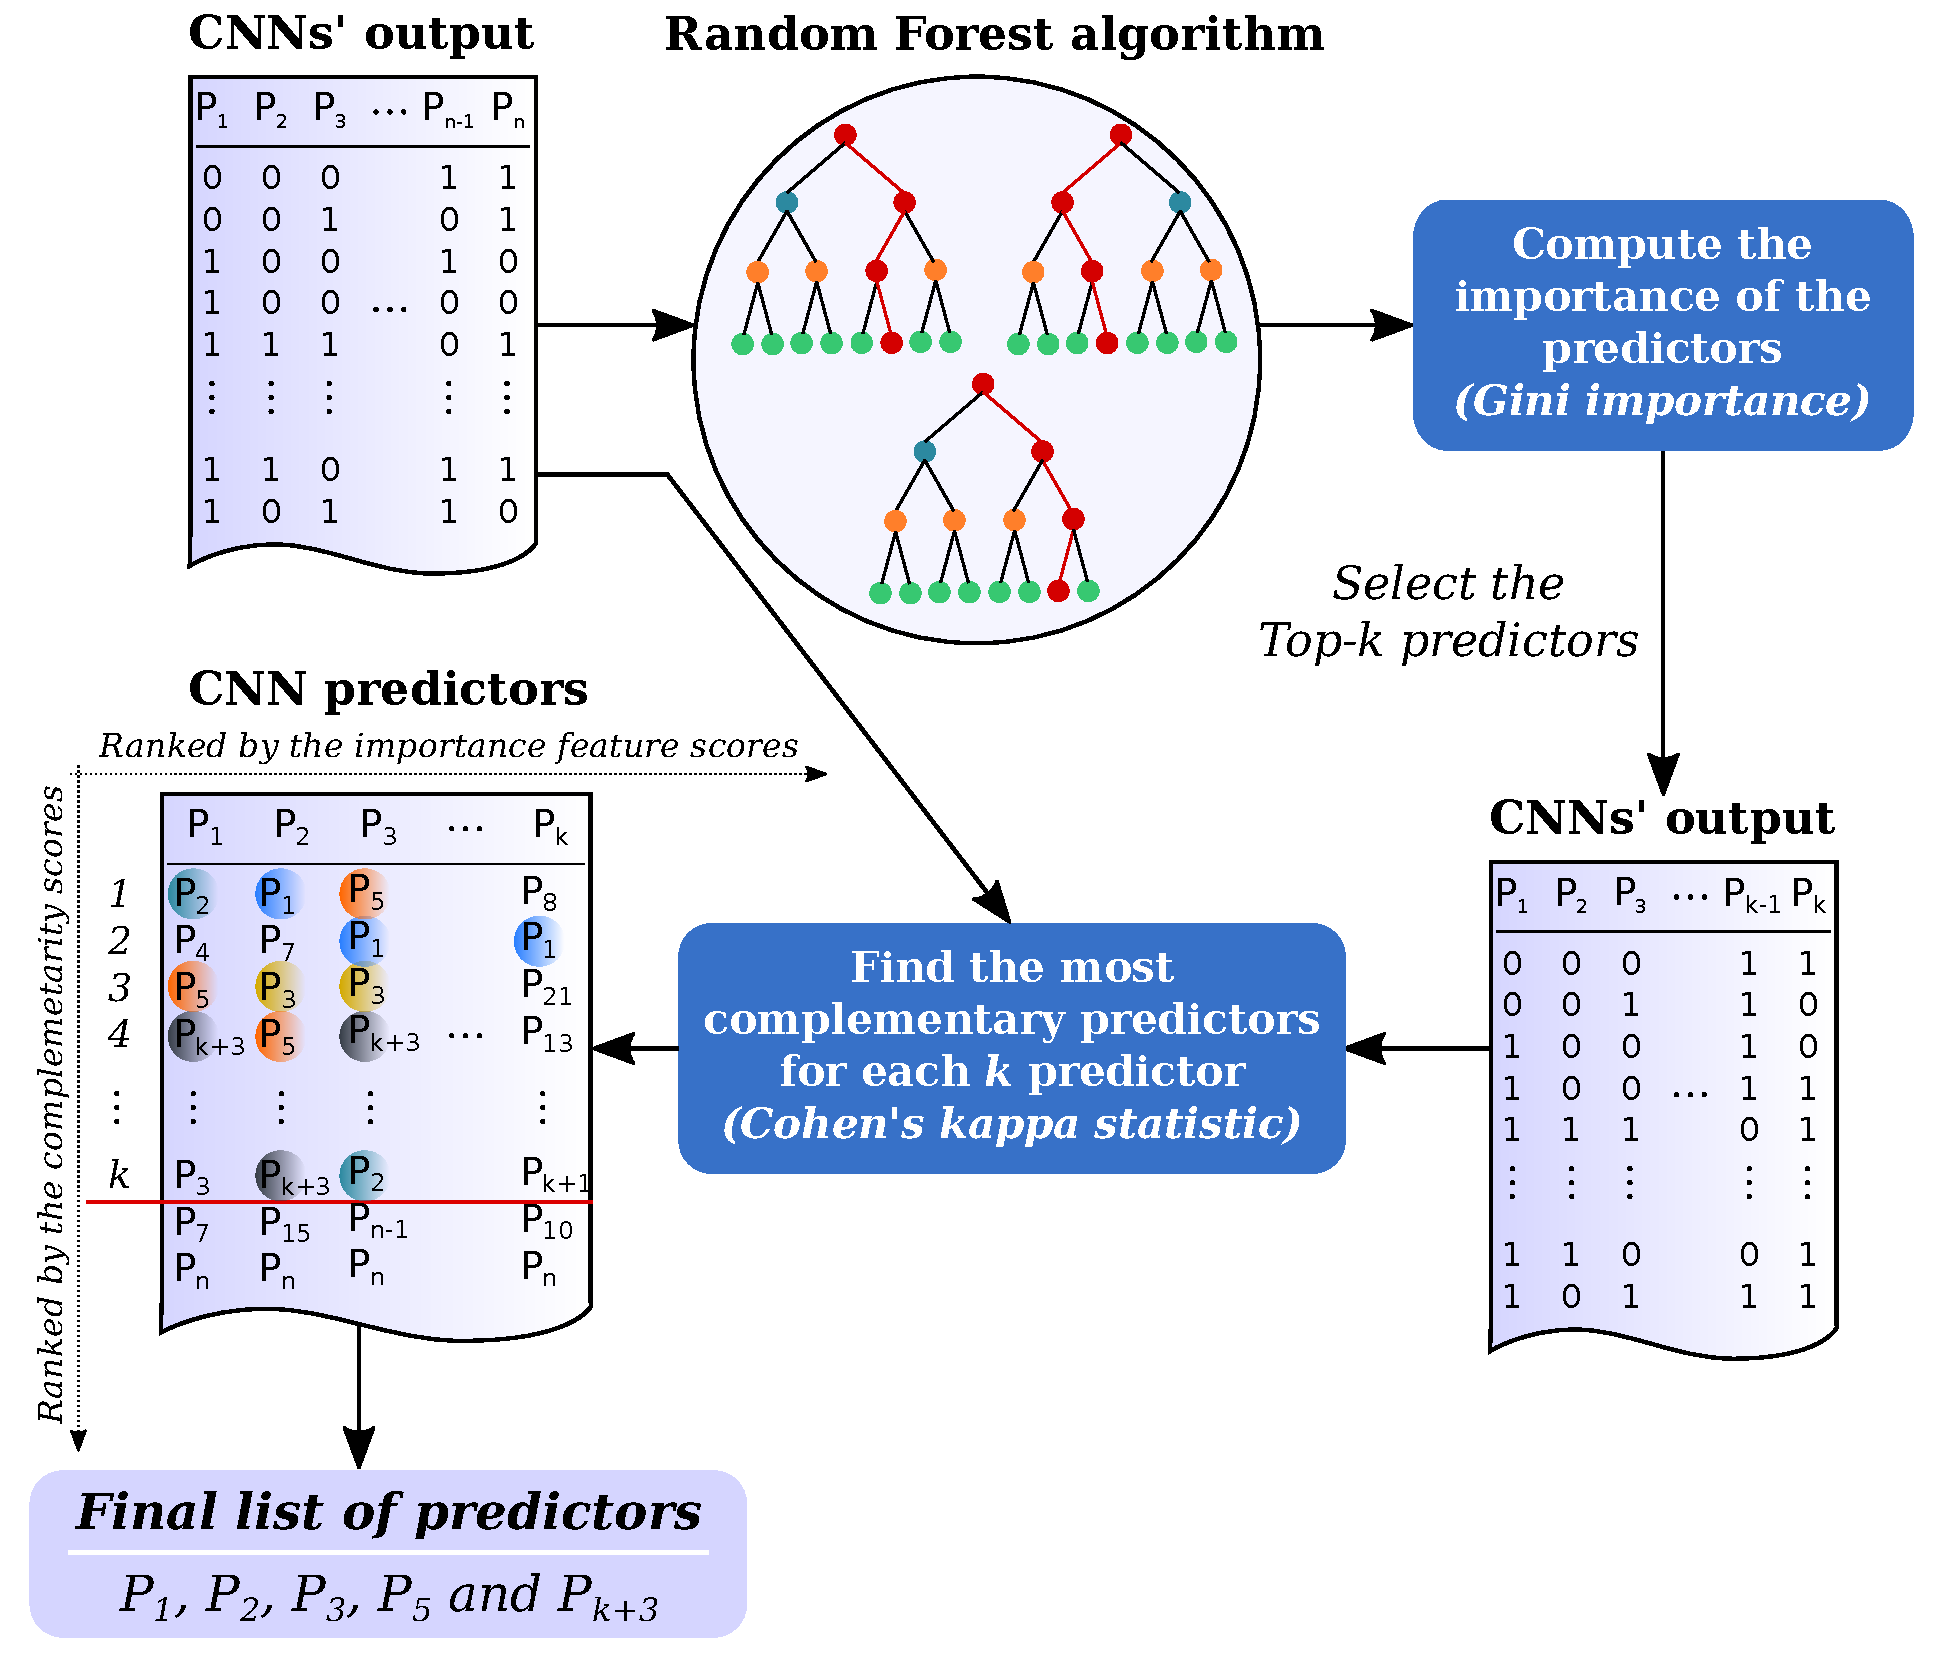
\includegraphics[width=0.99\linewidth]{graphics/selection-algo-v2.pdf}
    \caption{Proposed algorithm for selecting predictors: after generating CNN outputs, a Random Forest is trained on the binary results of all predictors (feature vector $v \in R^{61}$ dimensions), to rank predictors by importance. The most complementary to each of the $k$ most important predictors are calculated through Cohen's kappa statistic. Finally, a predictor list is generated by selecting those which appear in two or more columns in the calculated matrix.}
\label{fig:proposed_method_selection}
\end{figure}

Our algorithm performs a score analysis of all multi-view-CNN predictors' outputs using the Random Forest algorithm to find the $k$ most important predictors. This step focuses on which models are important in the classification task in terms of their {Gini} importance, also known as mean decrease in impurity (MDI)~\cite{Breiman:1984}. In the context of our meta-analysis, each node of a tree represents a single feature, which is the output of a given predictor.

{Gini} importance measures how much the predictors decrease the weighted impurity in a tree. More precisely, the RF algorithm is a collection of decision trees aiming at splitting the data into two branches so that similar patterns end up in the same branch. The RF algorithm computes, during the training process, how much each predictor decreases the weighted impurity in a tree, and this metric is used to measure the quality of such splits. Our proposed algorithm takes advantage of that by ranking the multi-view-CNN predictors according to this measure and selecting the top-\textit{k} predictors, which will be our initial pool of good candidates for the fusion step.

After finding the $k$ most important models, we compute, through the Cohen's kappa statistic, which gives an agreement estimation between two predictors, their $l$ most complementary predictors, ending up with a $k \times l$ matrix $\mathbf{C}$ of predictors. 
%We are interested in finding the most complementary predictors between the list of $k$ most important predictors and full set of 61 CNN models. 
We compute a final list of predictors by selecting those that appear in two or more columns of $\mathbf{C}$. The final decision-making is accomplished through SVM meta-fusion, which takes $k$ selected predictor outcomes as the input.